% main.tex -- ECON 20 final paper (JESAS group)
% Tables are \input from tables/ and figures from figures/. Both are copied from output/
% by build_overleaf.sh (the do-files and code/03_table1_format.py write them there).
% After rerunning the code: bash paper/build_overleaf.sh, then upload paper/overleaf.zip.
% Compile locally from this folder with: tectonic main.tex
\documentclass[12pt]{article}
\usepackage[margin=1in]{geometry}
\usepackage{amsmath}
\usepackage{graphicx}
\usepackage{setspace}
\usepackage{caption}
\usepackage{float}
\usepackage[hidelinks]{hyperref}
\usepackage{etoolbox}
\usepackage{adjustbox}
\AtBeginEnvironment{table}{\singlespacing}  % tables single-spaced
\graphicspath{{figures/}}
\captionsetup{labelfont=bf, font=small}
\onehalfspacing

% table notes: small text under a table
\newcommand{\tablenotes}[1]{\par\vspace{4pt}\begin{minipage}{0.95\textwidth}\footnotesize #1\end{minipage}}

\title{Did California's 2018 Board Gender Law (SB 826) Affect the Market Value of California-Headquartered Public Companies?}
\author{Seohee Cho \and Sophia Hinze \and Julian Nelson \and Ansh Oswal \and Eloise Riedel-Drouin}
\date{November 2026}

\begin{document}
\maketitle

%==============================================================================
\begin{abstract}
% TODO: 200--300 words. What we estimate and the basic findings.
\textit{Abstract goes here.}
\end{abstract}

%==============================================================================
\section{Introduction}

In recent years there has been a societal, political, and cultural push towards gender equity in the workplace, including prominent business positions such as the corporate board. Women's representation on corporate boards has risen steadily for more than a decade, and women now hold over one third of S\&P 500 board seats (Tonello \& Marchis-Mouren, 2025). On September 30 2018, California was the first US state to require women on corporate boards, signing SB 826 into law. SB 826 mandates that public corporations must have at least one woman director by December 31, 2019, and at a later date must meet a minimum percentage of women directors. By December 31, 2021, boards with five directors must include at least two women, and boards with six or more directors must include at least 3. SB 826 therefore provides an exogenous stimulus to the share of women on boards, raising the question of the resulting effect on market capitalization.

The economic arguments surrounding the effect of women directors revolve around financial consequences. Opponents of quotas argue that the number of qualified women directors is too small, and that an underqualified woman's appointment would harm the firm's financial performance. In Norway, the quota did lead to younger and less experienced boards (Ahern and Dittmar, 2012). Proponents of quotas argue that more diverse boards monitor managers more closely, which could raise firm value (Adams and Ferreira, 2009). A third possibility is that the law did little to change the share of women on boards. In Norway, penalties for failing to satisfy quotas gradually grew more extreme over a period of four years when companies that didn't comply were threatened with dissolution. SB 826, however, listed the penalty for non-compliance as \$100,000 for the first-time offense, and \$300,000 going forward.

We study this question with a difference-in-differences design that compares listed firms headquartered in California with listed firms headquartered in Texas. We use annual financial and stock market data from Compustat, merged with board composition data from BoardEx for fiscal years 2010 through 2019. Texas is a large state with many public companies and no board gender quota. Our outcome is the natural log of each firm's market capitalization at the fiscal year's end. Our main estimates compare two things: how California firms' market capitalization changed between fiscal year 2018, when the law was signed, and fiscal year 2019, when the first requirement took effect, with how Texas firms' market capitalization changed over those two years. We estimate this by ordinary least squares, with and without controls for firm size, profitability, leverage, and multinational status, and cluster standard errors by firm. For this comparison to measure the law's effect, the market capitalizations of California and Texas firms must have had parallel trajectories absent SB 826. We test this assumption with an event study from 2010 to 2018 that follows each firm over time, and because the test fails, we also report estimates that remove California's pre-law trend. As a placebo test, we repeat the analysis for firms that already had a woman director in 2018 since they were unbound by the 2019 requirement. Finally, we use the law as an instrument to estimate the value of adding women directors.

% TODO (required): paragraph summarizing the findings, with the size of the main estimates.

%==============================================================================
\section{Data \& Methods}

We used three datasets obtained from wharton.upenn.edu to construct our data. We first used the \textit{Compustat North America: Fundamentals Annual} (S\&P Global Market Intelligence, 2026) dataset from 2010--2019 for the states of California and Texas. This data set gives us access to financial statements and market caps for public companies. Our second dataset is \textit{BoardEx North America, Organization Summary -- Analytics} (BoardEx, 2026). This data set gives us board size and gender ratio (which we pull from each annual report) for each public company from 2010--2019 in California and Texas. Our third dataset is \textit{WRDS BoardEx--CRSP--Compustat link table} (Wharton Research Data Services, 2026) which matches the BoardEx company IDs to the Compustat company IDs. From these, we only kept data from publicly traded companies from 2010--2019 in California and Texas.

To analyze the impact of the California's Women on Boards law (SB 826) on market capitalization in California we use the following estimation equation:
\begin{equation}
\ln(\text{mktcap})_{it} = b_0 + b_1 \text{Post}_t + b_2 (\text{CA}_i \times \text{Post}_t) + a_i + u_{it}
\label{eq:did}
\end{equation}
Our dependent variable is the log market cap of a certain company $i$ at year $t$ (\texttt{lnmktcap} in our code). We estimate this using two variables: California ($\text{CA}_i$), a dummy indicating whether a company is based in California (instead of Texas) and a dummy variable for after the policy (Post) which equals 1 if the firm's fiscal year ended on or after October 1, 2018, the day after SB 826 was signed into law, and 0 otherwise. The California main effect is omitted since we control for company fixed effects ($a_i$). The means and standard deviations of the main variables used in the analysis are shown in Table~\ref{tab:means}.

We assume that absent the Women on Boards law in California, the market capitalization of companies would have increased by the same proportion in California and Texas. We calculate our standard errors to be robust to heteroskedasticity and autocorrelation by clustering on companies.

Ultimately we are interested in whether gender composition of the board affects the market capitalization of a given company. To identify that we undertake an instrumental variables approach where the law (CA $\times$ Post) serves as an instrument for the dummy variable indicating whether a company has at least one woman on the board (OneWm). We assume that the Women on Boards law is correlated with having at least one woman on the board. To check this we use the first stage equation:
\begin{equation}
\text{OneWm}_{it} = b_0 + b_1 \text{Post}_t + b_2 (\text{CA}_i \times \text{Post}_t) + a_i + u_{it}
\label{eq:fs}
\end{equation}
Our second assumption is that CA $\times$ Post is uncorrelated with any third factors (other than OneWm) that affect the market capitalization of a company. From these we calculate our reduced form, equation~(\ref{eq:did}). Using indirect least squares we can then calculate our IV slope coefficient which gives us the effect of OneWm on market capitalization.

%------------------------------------------------------------------------------
\begin{table}[H]
\centering
\caption{Means and Balance Test: California vs.\ Texas, Before and After SB 826}
\label{tab:means}
\adjustbox{max width=\textwidth, max height=0.62\textheight}{\begin{tabular}{lcccccc}
\hline\hline
 & \multicolumn{2}{c}{Before the law} & \multicolumn{2}{c}{After the law} & CA $-$ TX & Difference- \\
\cline{2-3} \cline{4-5}
 & Texas & California & Texas & California & before & in-differences \\
 & (1) & (2) & (3) & (4) & (5) & (6) \\
\hline
\multicolumn{7}{l}{\textit{Panel A. Outcome and board composition}} \\
Ln(market cap) & 6.761 & 6.456 & 6.527 & 7.079 &  &  \\
 & [2.095] & [2.180] & [2.136] & [2.307] &  &  \\
Women on board & 0.887 & 0.998 & 1.458 & 1.976 &  &  \\
 & [0.960] & [1.009] & [1.121] & [1.083] &  &  \\
No women on board & 0.423 & 0.374 & 0.197 & 0.046 &  &  \\
 & [0.494] & [0.484] & [0.398] & [0.210] &  &  \\
\multicolumn{7}{l}{\textit{Panel B. Firm characteristics (balance test)}} \\
Ln(total assets) & 6.979 & 6.184 & 6.942 & 6.555 & -0.794 & 0.408 \\
 & [2.197] & [2.186] & [2.238] & [2.192] & (0.137) & (0.084) \\
Net income / total assets & -0.041 & -0.156 & -0.088 & -0.163 & -0.115 & 0.039 \\
 & [0.730] & [0.576] & [0.331] & [0.477] & (0.023) & (0.025) \\
Total liabilities / total assets & 0.562 & 0.510 & 0.591 & 0.520 & -0.052 & -0.018 \\
 & [0.368] & [0.380] & [0.422] & [0.377] & (0.018) & (0.021) \\
Multinational (foreign income) & 0.385 & 0.561 & 0.381 & 0.555 & 0.176 & -0.003 \\
 & [0.487] & [0.496] & [0.486] & [0.497] & (0.029) & (0.022) \\
\quad \textit{Foreign income not reported} & 0.575 & 0.402 & 0.571 & 0.389 & -0.173 & -0.009 \\
 & [0.494] & [0.490] & [0.495] & [0.488] & (0.029) & (0.022) \\
Years since IPO & 11.73 & 10.94 & 13.52 & 10.25 & -0.80 & -2.46 \\
 & [9.15] & [8.77] & [10.80] & [10.10] & (0.68) & (0.55) \\
\quad \textit{IPO date missing} & 0.429 & 0.309 & 0.425 & 0.282 & -0.121 & -0.022 \\
 & [0.495] & [0.462] & [0.495] & [0.450] & (0.030) & (0.018) \\
Listed on NYSE & 0.521 & 0.229 & 0.476 & 0.240 & -0.292 & 0.056 \\
 & [0.500] & [0.420] & [0.500] & [0.427] & (0.029) & (0.018) \\
Tech sector (GICS 45) & 0.101 & 0.338 & 0.095 & 0.260 & 0.238 & -0.072 \\
 & [0.301] & [0.473] & [0.293] & [0.439] & (0.024) & (0.016) \\
Oil and gas (SIC 13, 29) & 0.242 & 0.005 & 0.235 & 0.005 & -0.236 & 0.006 \\
 & [0.428] & [0.074] & [0.424] & [0.068] & (0.021) & (0.012) \\
Board size & 8.18 & 8.04 & 8.12 & 8.32 & -0.14 & 0.34 \\
 & [2.35] & [1.96] & [2.37] & [1.97] & (0.14) & (0.10) \\
Pharma or biotech (SIC 2833-2836) & 0.027 & 0.195 & 0.048 & 0.253 &  &  \\
 & [0.163] & [0.397] & [0.213] & [0.435] &  &  \\
\hline
Firm-years & 3,104 & 4,011 & 776 & 1,080 & 7,115 & 8,971 \\
Firms & 547 & 753 & 412 & 600 & 1,300 & 1,470 \\
\hline\hline
\end{tabular}
}
\tablenotes{Notes: Sample is firms headquartered in California or Texas on 30 September 2018, listed on the NYSE, AMEX or Nasdaq, excluding funds, trusts and shell companies (SIC 67xx) and firm-years with under \$1 million of total assets. ``Before'' is fiscal years ending January 2011 to September 2018; ``After'' is fiscal years ending October 2018 to December 2020. Columns (1)--(4) report unweighted means with standard deviations in brackets. Column (5) is the coefficient on a California dummy from a regression of the row variable on that dummy, before-the-law sample only. Column (6) is the coefficient on California $\times$ After from a regression of the row variable on California, After and their interaction, full sample. Standard errors in columns (5) and (6) are in parentheses and clustered by firm. Market cap is fiscal-year-end price times shares outstanding. Multinational equals 1 if Compustat reports nonzero foreign pretax income; blank values are counted as zero, and the share blank is shown in the row below. Years since IPO is missing where Compustat has no IPO date (mostly older firms); the share missing is shown in the row below. Board variables are from BoardEx and are available for 85 percent of firm-years. Sources: Compustat North America Fundamentals Annual and BoardEx North America, via WRDS.}
\end{table}

Table~\ref{tab:means} reports means and a balance test for the firm characteristics we consider for controls. Before the law (column 5), California firms were smaller (ln assets 0.79 lower), less profitable (net income over assets 10 percentage points lower), and slightly less leveraged (liabilities over total assets 5 percentage points lower). They were also more often in technology (35 versus 10 percent), almost never in oil and gas (1 versus 24 percent), and less often listed on the NYSE (22 versus 52 percent). They were more likely to report foreign income (56 versus 38 percent), though Texas firms also leave that field blank more often. Firm age and board size did not differ significantly. These differences in initial characteristics do not threaten our design by themselves since the assumption is parallel trends, not parallel levels. We also include firm fixed effects to remove any fixed differences between firms.

We test whether characteristics changed differently after the law with column (6). Seven of the nine characteristics show no statistically significant differential change. The exceptions are technology share, which fell 8.8 percentage points more in California relative to Texas, and years since IPO, which fell 1.9 years more in California relative to Texas. The differential change in technology share and firm age suggests that California firms became younger and shifted away from technology after 2018 (consistent with the entrance of biotech firms). This could threaten parallel trends, but only if these firms' stock prices follow different trends from others.

We address these changes in firm characteristics through firm fixed effects and time-varying controls. Firm fixed effects absorb all characteristics that are constant within firms. We also control for time-varying characteristics like log total assets, net income over total assets, liabilities over total assets, and multinational status. These controls, however, do not fully address the compositional shift which is a result only of firms entering or leaving the sample. As a robustness check, we include only the balanced panel of 824 firms that were observed before and after the law.

%==============================================================================
\section{Results}

%------------------------------------------------------------------------------
\begin{table}[H]
\centering
\caption{Pre-trends: California $\times$ year, relative to 2018}
\label{tab:pretrend}
\small
\begin{tabular}{lc} \hline
 & (1) \\
VARIABLES & (1) Pretrend coefficients \\ \hline
 &  \\
ca\_yr2011 & -0.595*** \\
 & (0.106) \\
ca\_yr2012 & -0.629*** \\
 & (0.095) \\
ca\_yr2013 & -0.622*** \\
 & (0.086) \\
ca\_yr2014 & -0.397*** \\
 & (0.077) \\
ca\_yr2015 & -0.122* \\
 & (0.072) \\
ca\_yr2016 & -0.273*** \\
 & (0.069) \\
ca\_yr2017 & -0.137*** \\
 & (0.048) \\
Constant & 6.607*** \\
 & (0.069) \\
 &  \\
Observations & 7,115 \\
R-squared & 0.938 \\
Firm FE & Yes \\
 Year FE & Yes \\ \hline
\multicolumn{2}{c}{ Robust standard errors in parentheses} \\
\multicolumn{2}{c}{ *** p$<$0.01, ** p$<$0.05, * p$<$0.1} \\
\end{tabular}

\tablenotes{Notes: Standard errors in parentheses are robust to autocorrelation within firms and to heteroskedasticity.}
\end{table}

We observe the difference in the market cap of companies in both California and Texas before the Senate Bill came into effect. From Table~\ref{tab:pretrend} we notice that in the years leading up to 2018 (2010--2017), the market cap between California and Texas was significantly different than in our reference year (2018). We find that every year (except 2015) is significantly different at the 0.01 significance level. We also see that the differences between California and Texas change over the years. Indeed, this difference in log market cap is .605 log points ($\sim$45\%) lower in 2011 than in 2018 but only .137 log points ($\sim$13\%) lower in 2017 than in 2018. This indicates that before the Senate Bill passed, market caps of companies in California and Texas were following different trajectories. This brings up an important issue as we cannot assume that the pretrends were insignificant.

\begin{figure}[H]
\centering
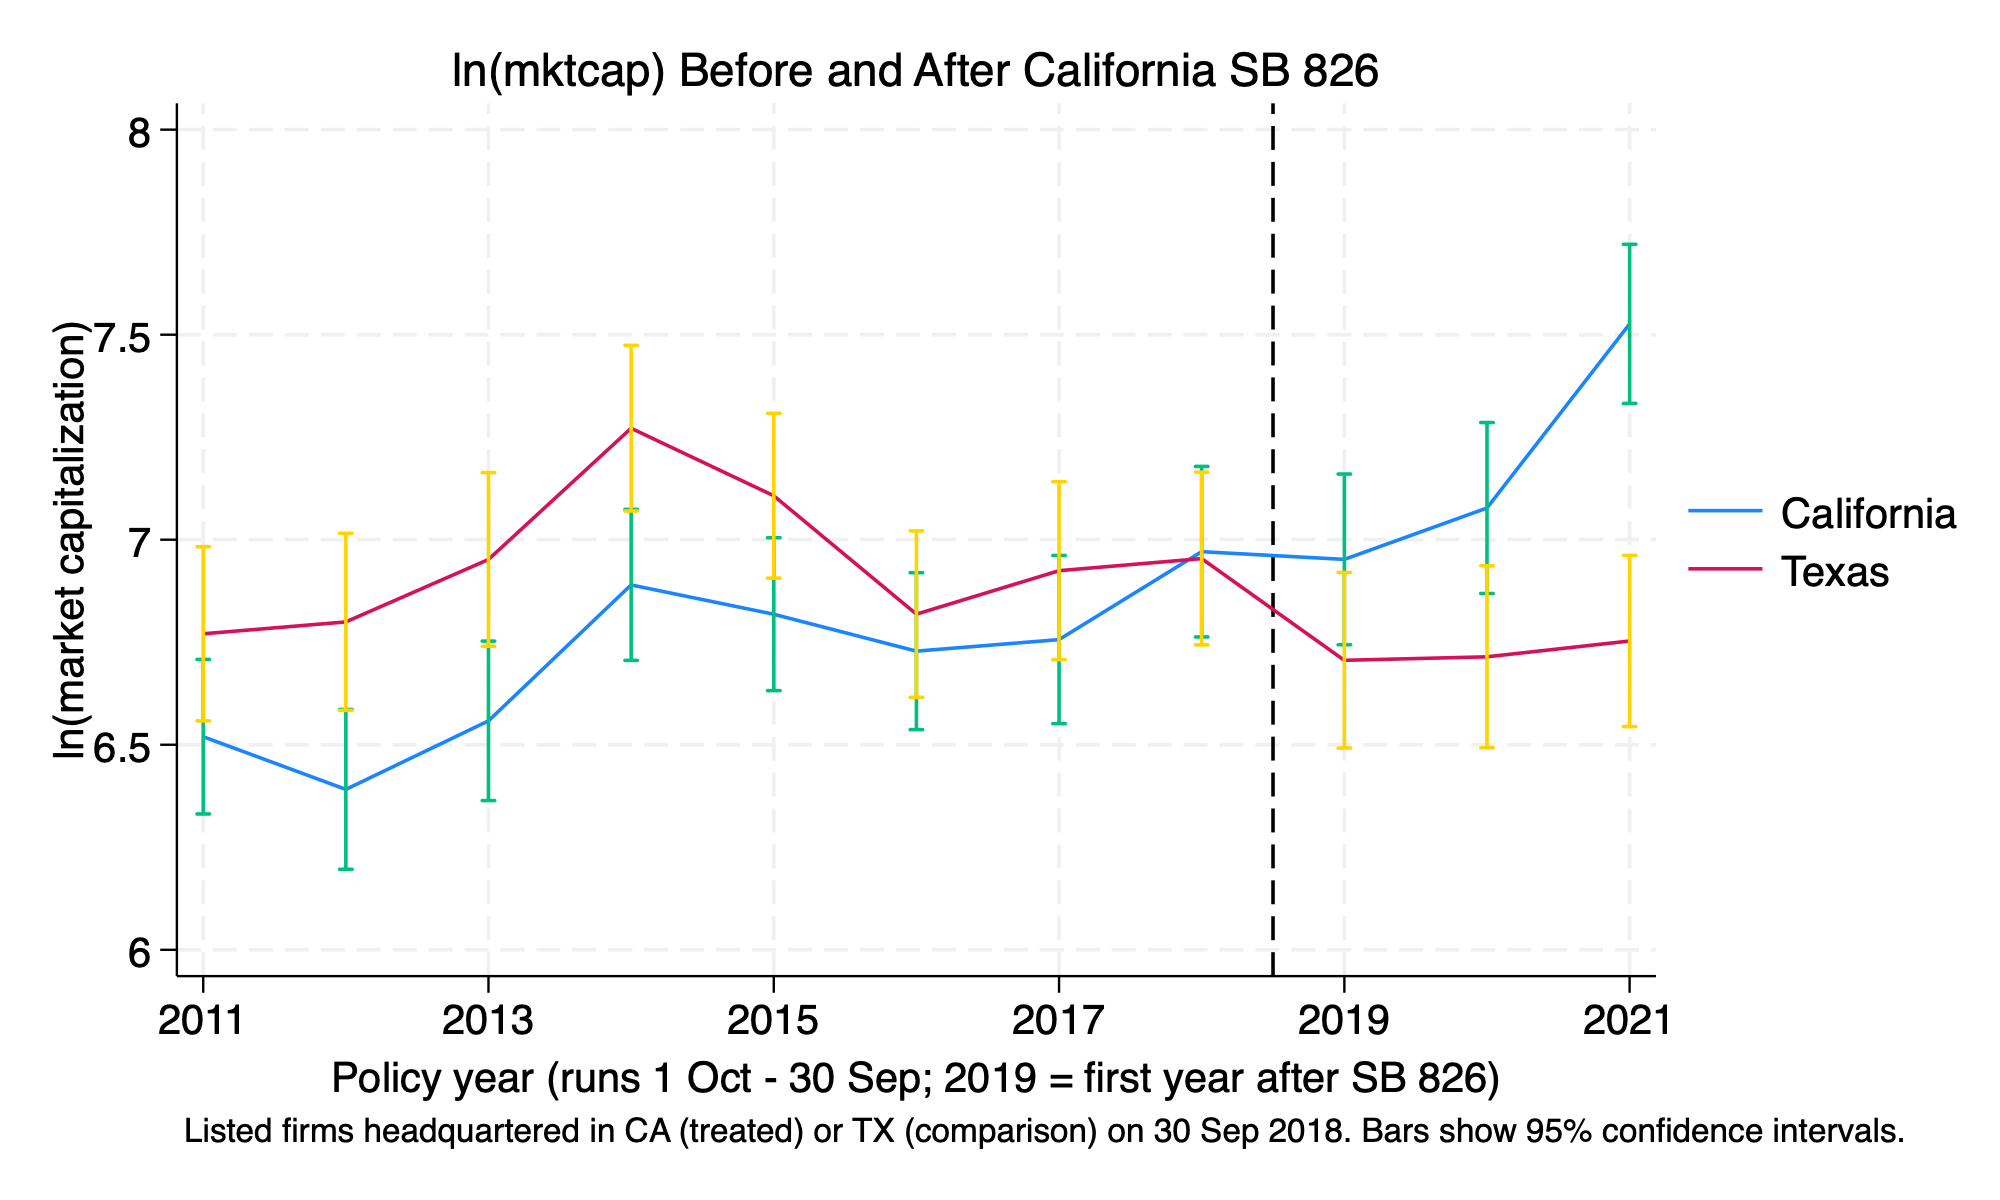
\includegraphics[width=\textwidth]{doc_means_lnmktcap_2021.png}
\caption{Pre-trend: ln(market cap) before and after SB 826, California vs.\ Texas}
\label{fig:pretrend}
\end{figure}

Figure~\ref{fig:pretrend} demonstrates how California firms' market capital were catching up to the level of Texas' before SB 826 was implemented around 2018. Since this shrinking gap violates the parallel trends assumption, detrending was used to estimate the pure effect of SB 826 by observing the divergence from what the pre-trend alone would predict.

%------------------------------------------------------------------------------
\begin{table}[H]
\centering
\caption{Event study, CA $\times$ each year, relative to 2017, 2011--2020}
\label{tab:eventstudy}
\adjustbox{max width=\textwidth, max height=0.75\textheight}{\begin{tabular}{lcccc} \hline
 & (1) & (2) & (3) & (4) \\
 & (1) First stage & (2) First stage & (3) Reduced form & (4) Reduced form \\
VARIABLES & One woman & One woman & ln(mkt cap) & ln(mkt cap) \\ \hline
 &  &  &  &  \\
caXyr2011 & -0.031 & 0.048 & -0.416*** & 0.175** \\
 & (0.041) & (0.041) & (0.085) & (0.085) \\
caXyr2012 & -0.049 & 0.017 & -0.476*** & 0.017 \\
 & (0.039) & (0.039) & (0.077) & (0.077) \\
caXyr2013 & -0.073** & -0.020 & -0.434*** & -0.040 \\
 & (0.036) & (0.036) & (0.068) & (0.068) \\
caXyr2014 & -0.059* & -0.019 & -0.222*** & 0.074 \\
 & (0.032) & (0.032) & (0.061) & (0.061) \\
caXyr2015 & -0.044 & -0.018 & 0.002 & 0.199*** \\
 & (0.028) & (0.028) & (0.054) & (0.054) \\
caXyr2016 & -0.016 & -0.003 & -0.162*** & -0.063 \\
 & (0.022) & (0.022) & (0.040) & (0.040) \\
caXyr2018 & -0.008 & -0.021 & 0.211*** & 0.112** \\
 & (0.023) & (0.023) & (0.045) & (0.045) \\
caXyr2019 & 0.049 & 0.023 & 0.264*** & 0.067 \\
 & (0.032) & (0.032) & (0.060) & (0.060) \\
caXyr2020 & 0.022 & -0.017 & 0.721*** & 0.426*** \\
 & (0.035) & (0.035) & (0.078) & (0.078) \\
Constant & 0.903*** & 0.361*** & 6.798*** & -0.049 \\
 & (0.025) & (0.025) & (0.054) & (0.054) \\
 &  &  &  &  \\
Observations & 7,906 & 7,906 & 7,906 & 7,906 \\
R-squared & 0.172 & 0.174 & 0.161 & 0.032 \\
Number of firm\_id & 1,301 & 1,301 & 1,301 & 1,301 \\
Firm FE & Yes & Yes & Yes & Yes \\
Year FE & Yes & Yes & Yes & Yes \\
Detrended & No & Yes & No & Yes \\
Joint pre-trend F & 1.015 & 1.165 & 14.92 & 12.19 \\
 Joint pre-trend p & 0.414 & 0.322 & 0 & 0 \\ \hline
\multicolumn{5}{c}{ Robust standard errors in parentheses} \\
\multicolumn{5}{c}{ *** p$<$0.01, ** p$<$0.05, * p$<$0.1} \\
\end{tabular}
}
\tablenotes{Notes: Standard errors in parentheses are robust to autocorrelation within firms and to heteroskedasticity. 2017 is the omitted year.}
\end{table}

Table~\ref{tab:eventstudy} reports the event-study coefficients that are plotted in Figures~\ref{fig:fs} and~\ref{fig:rf}. Each coefficient is the difference between California and Texas firms in a given fiscal year, relative to the same difference in fiscal year 2017, the last fully pre-law year. We use 2017 rather than 2018 because about 80 percent of fiscal-year-2018 observations end after the law was signed, so 2018 is a partly treated year. All specifications include firm and year fixed effects, with standard errors clustered by firm. Columns (1) and (2) use the probability that a board has at least one woman as the outcome (first stage), and columns (3) and (4) use ln(market cap) (reduced form). Columns (2) and (4) subtract California's linear pre-law trend from the outcome. The bottom rows report a joint F-test that all pre-law coefficients equal zero.

\begin{figure}[H]
\centering
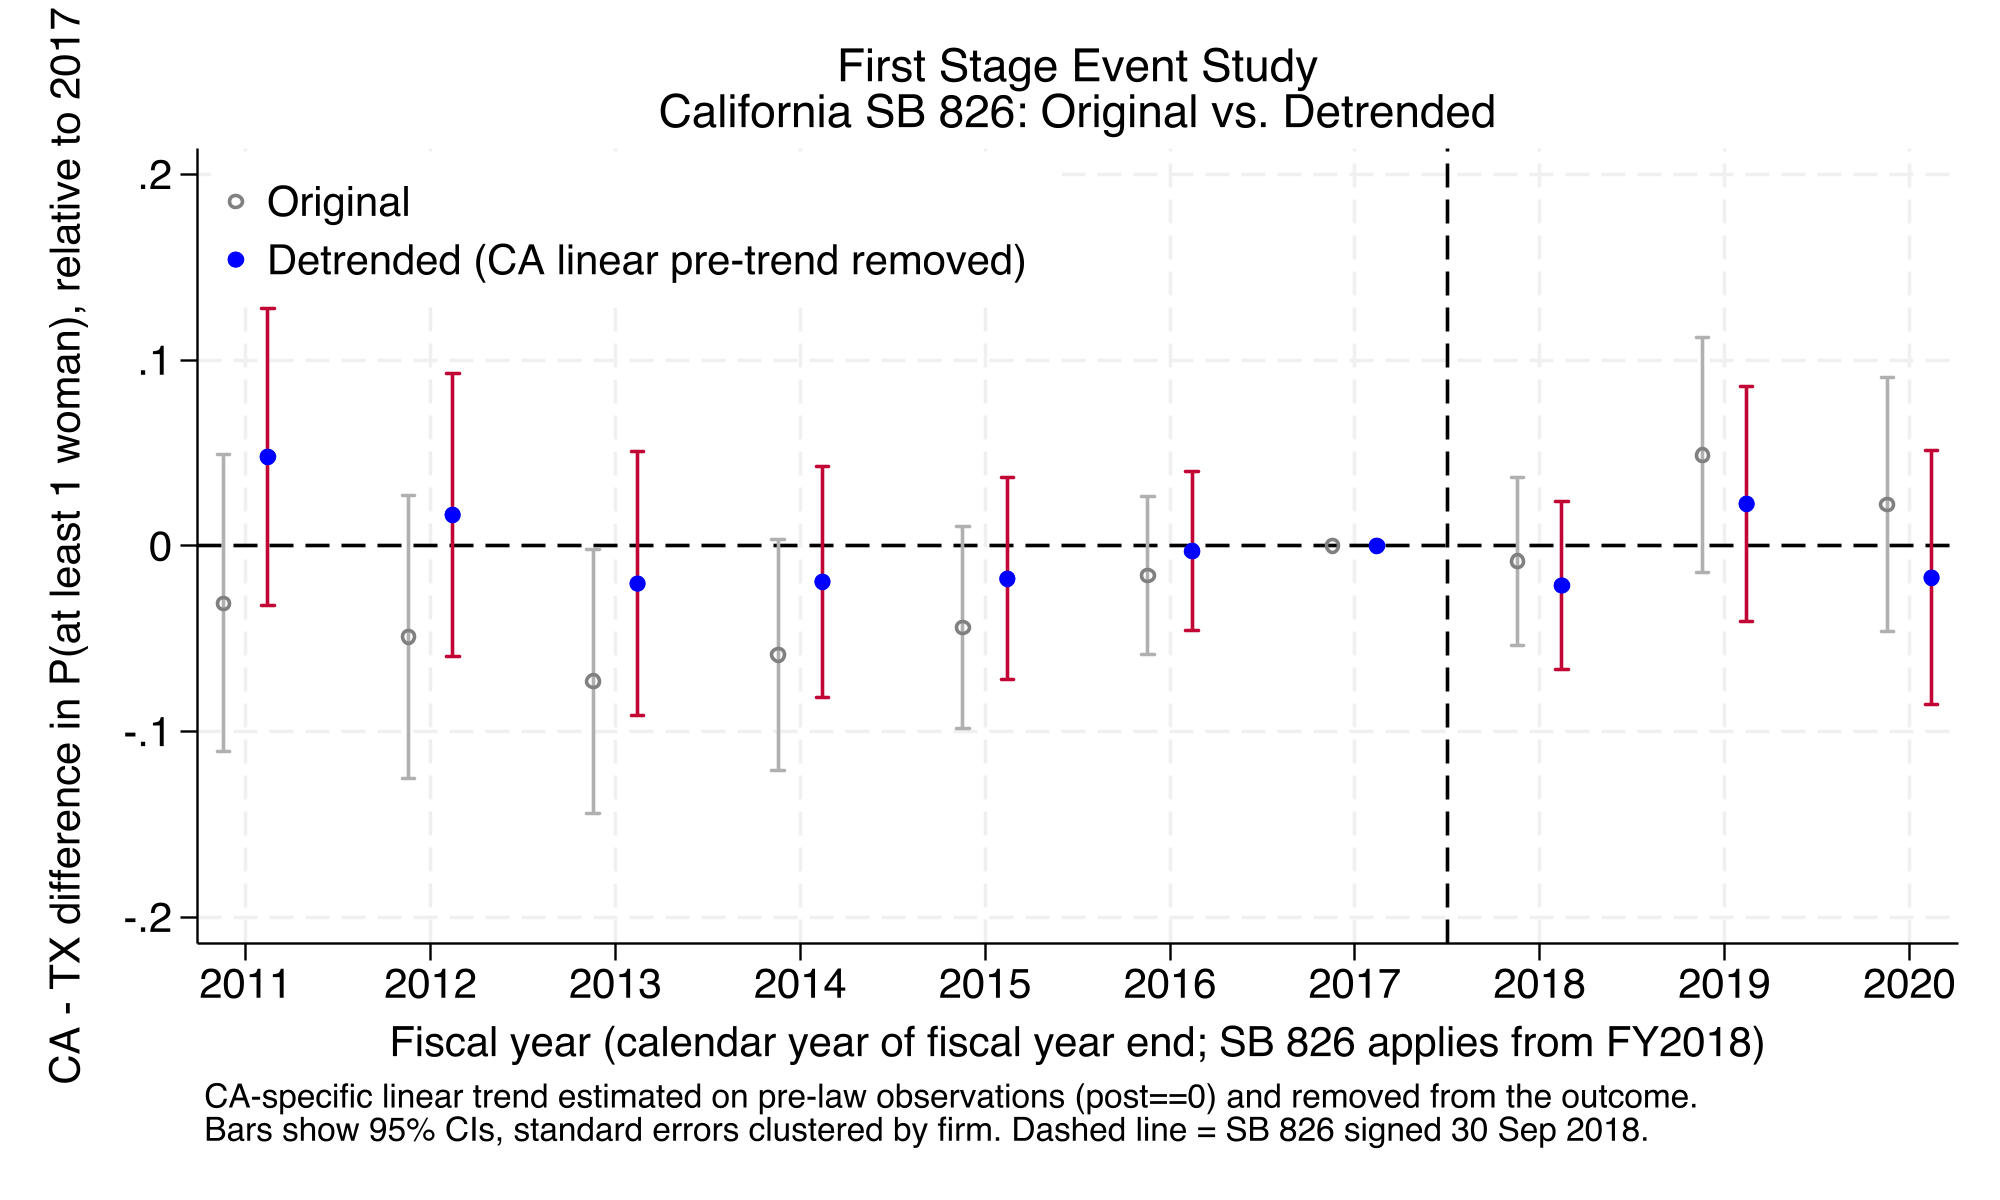
\includegraphics[width=\textwidth]{es_onewoman_overlay.png}
\caption{First Stage Event Study}
\label{fig:fs}
\end{figure}

Columns (1) and (2) of Table~\ref{tab:eventstudy} and Figure~\ref{fig:fs} show no significant (at the 1\% level) effect of SB 826 on whether a firm has at least one woman on its board. In the original specification, all six pre-law coefficients are negative, between -0.017 and -0.074, and they drift toward zero by 2017. Only 2013 (-0.074) and 2014 (-0.058) are individually significant, at the 5 and 10 percent levels, so we find no statistical evidence of a differential pre-trend in having at least one woman on board between California and Texas before SB 826 (F = 1.026, p = 0.407 in the original specification; F = 0.976, p = 0.440 after detrending). After detrending, the pre-law coefficients range from -0.039 to 0.020, and none is significant (joint F = 0.976, p = 0.440). After the law, the original estimates are -0.008 in 2018, 0.048 in 2019, 0.023 in 2020, and 0.011 in 2021, and the detrended estimates are -0.017, 0.031, -0.003, and -0.024. None is statistically significant in either specification. SB 826 therefore did not change the share of California firms with at least one woman on the board relative to Texas, which is consistent with most large firms already meeting the law's minimum requirement. This is also why the dummy measure gives a weak first stage in the IV and why we use the share of women as our main measure.

\begin{figure}[H]
\centering
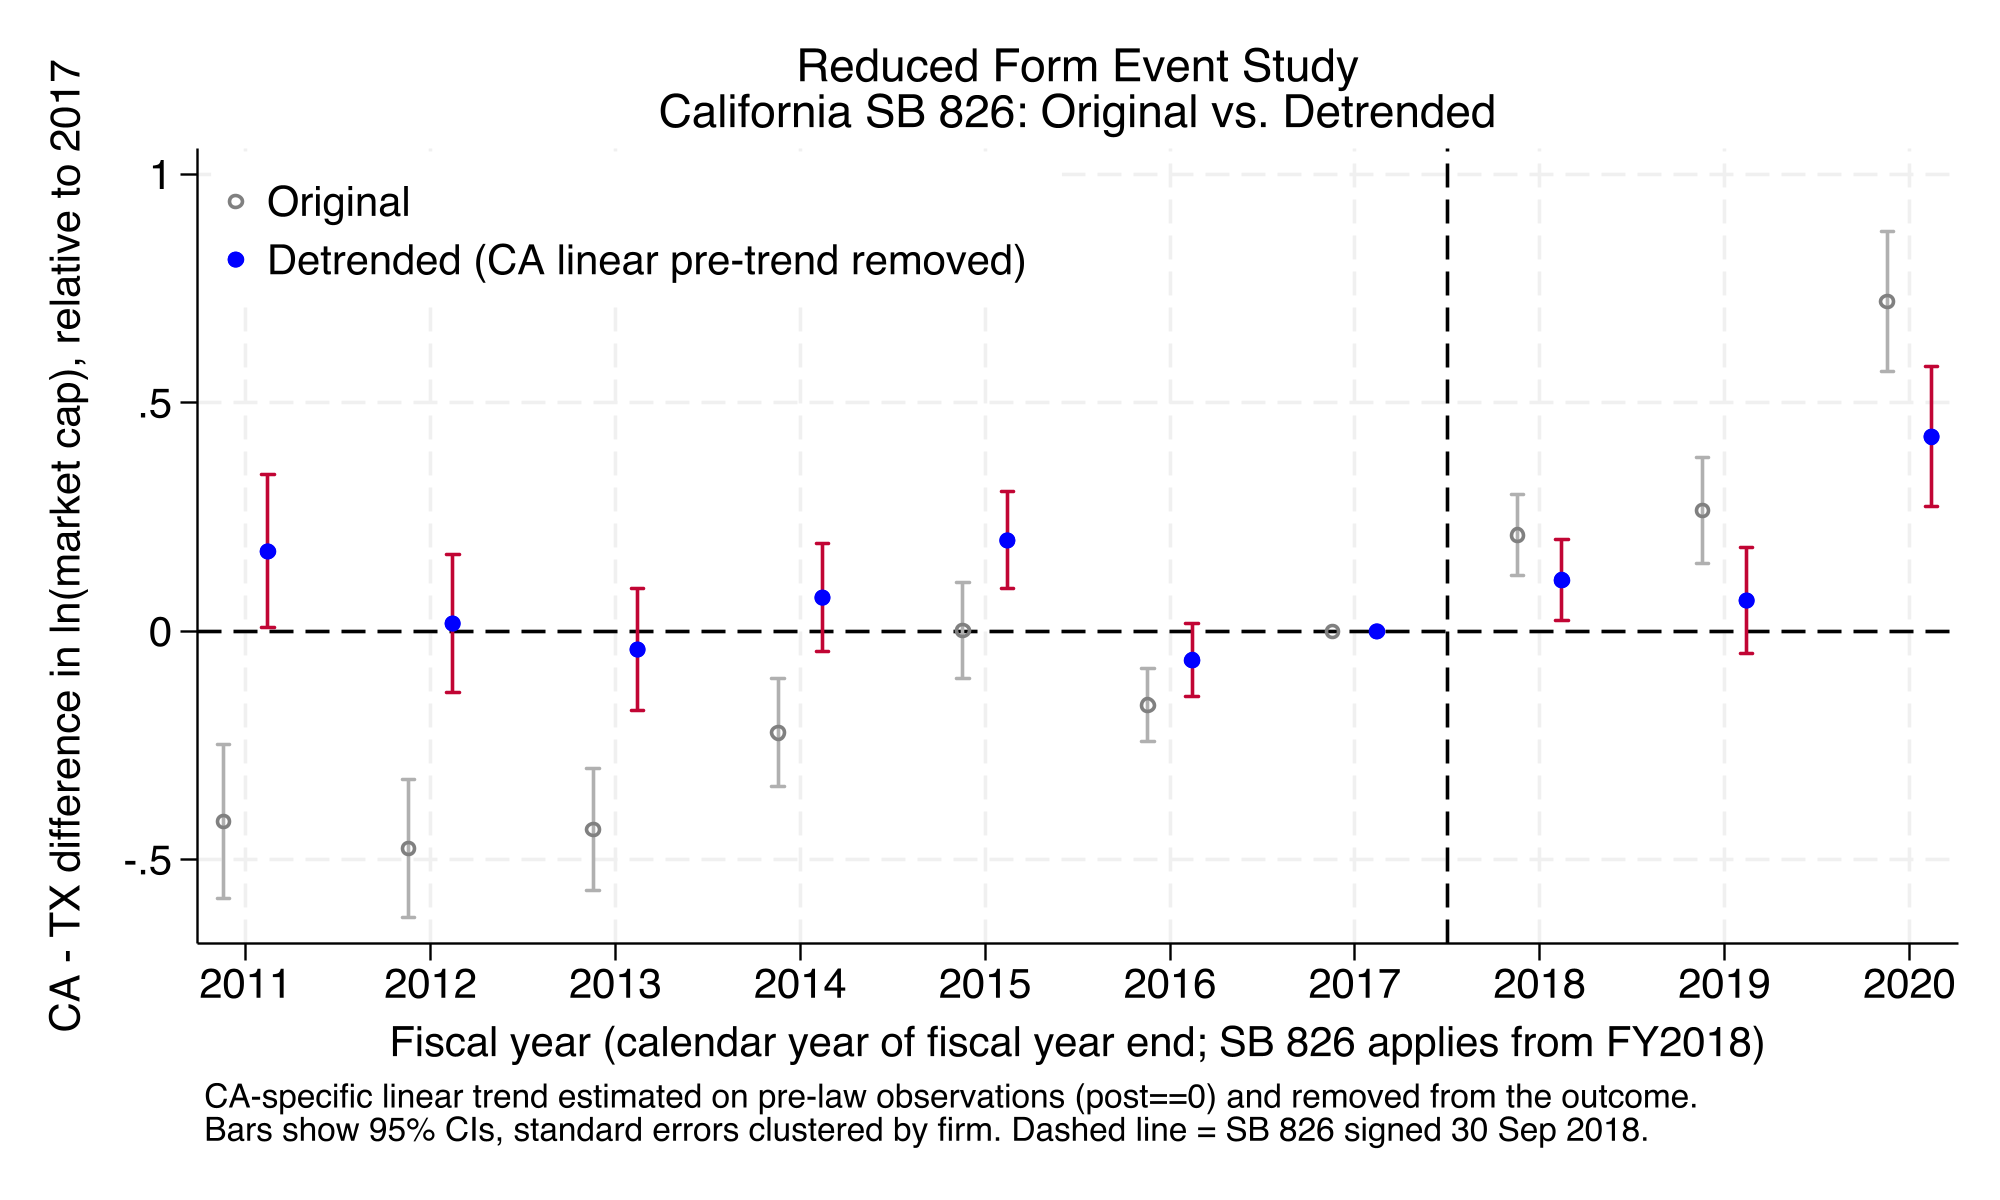
\includegraphics[width=\textwidth]{es_lnmktcap_overlay.png}
\caption{Reduced Form Event Study}
\label{fig:rf}
\end{figure}

Columns (3) and (4) of Table~\ref{tab:eventstudy} and Figure~\ref{fig:rf} show a large pre-trend in market capitalization that detrending reduces but does not eliminate. In the original specification, the pre-law coefficients are negative and significant at the 1 percent level in every year except 2015: -0.410 in 2011, -0.471 in 2012, -0.431 in 2013, -0.218 in 2014, and -0.159 in 2016. This confirms that California firms were catching up to Texas firms before the law, and the joint test strongly rejects parallel trends (F = 14.58, p $<$ 0.001). After detrending, the pre-law coefficients no longer drift in one direction 0.077 in 2011, -0.064 in 2012, -0.106 in 2013, 0.026 in 2014, 0.167 in 2015, and -0.07 in 2016. Although 2015 (1 percent level) and 2016 (10 percent level) remain individually significant, we can say that there is statistical evidence a differential pre-trend in log market capitalization between California and Texas followed parallel trends before SB 826 (F = 11.40, p $<$ 0.001) and detrending reduces but does not clearly eliminates. After the law, the original estimates are positive and significant at the 1 percent level: 0.211 in 2018, 0.266 in 2019, 0.726 in 2020, and 0.566 in 2021. Detrending shrinks them to 0.129 (2018), 0.103 (2019, significant at the 10 percent level), 0.482 (2020), and 0.241 (2021). A positive gap therefore remains, roughly 62 percent in 2020 and 27 percent in 2021 ($\exp(\beta) - 1$), but a large part of the raw gap reflects California's earlier trend. Because the first stage shows no change in having at least one woman on the board, this gap is unlikely to operate through board composition. It may instead reflect other California-specific factors, such as shocks that coincide with the 2020--2021 period, which is the limitation we discuss in the IV section.

%------------------------------------------------------------------------------
\begin{table}[H]
\centering
\caption{Two-period DiD, FY2018 vs.\ FY2019}
\label{tab:did}
\small
\begin{tabular}{lcccc} \hline
 & (1) & (2) & (3) & (4) \\
VARIABLES & (1) lnmktcap & (2) lnmktcap & (3) lnmktcap & (4) lnmktcap \\ \hline
 &  &  &  &  \\
ca & 0.105 & 0.471*** & 0.184 & 0.551*** \\
 & (0.148) & (0.073) & (0.148) & (0.073) \\
post19 & 0.055 & 0.023 & 0.055 & 0.023 \\
 & (0.044) & (0.033) & (0.044) & (0.033) \\
ca\_post19 & 0.168*** & 0.122*** & 0.096 & 0.049 \\
 & (0.062) & (0.043) & (0.062) & (0.043) \\
lnassets &  & 0.850*** &  & 0.850*** \\
 &  & (0.020) &  & (0.020) \\
roa &  & -0.053 &  & -0.053 \\
 &  & (0.083) &  & (0.083) \\
leverage &  & -0.611*** &  & -0.611*** \\
 &  & (0.168) &  & (0.168) \\
multinational &  & 0.635*** &  & 0.635*** \\
 &  & (0.070) &  & (0.070) \\
Constant & 6.566*** & 0.743*** & -0.115 & -5.939*** \\
 & (0.106) & (0.126) & (0.106) & (0.126) \\
 &  &  &  &  \\
Observations & 1,799 & 1,789 & 1,799 & 1,789 \\
R-squared & 0.003 & 0.779 & 0.003 & 0.779 \\
Controls & No & Yes & No & Yes \\
 Detrended & No & No & Yes & Yes \\ \hline
\multicolumn{5}{c}{ Robust standard errors in parentheses} \\
\multicolumn{5}{c}{ *** p$<$0.01, ** p$<$0.05, * p$<$0.1} \\
\end{tabular}

\tablenotes{Notes: Standard errors in parentheses are robust to autocorrelation within firms and to heteroskedasticity.}
\end{table}

We observe the difference in the change of company market caps between California and Texas companies before and after the Senate Bill came into effect. Table~\ref{tab:did} shows that our interaction term is significant at the 1\% level in column 1 and 2. We see that absent detrending and controls (column 1) there is a 16.8\% higher change in market capitalization for Californian companies as opposed to Texan companies from 2018 to 2019. However, when accounting for past trends and controls we see that the difference in change between Californian and Texan company market capitalization drops to 6.2\%. We must account for the preexistent difference in trends because, as we saw in Table~\ref{tab:pretrend}, the pretrends differ quite significantly. To undertake our detrending we estimate a California specific time trend using the fiscal years preceding the passing of the law from 2010--2017, controlling for year fixed effects. We then project this trend forward and subtract it from the difference in log market capitalization found. Thus, the detrended coefficients measure the deviation from the path California was already on. By re-estimating this difference in difference, we can isolate the post law effect from the earlier trends. We see that the coefficient for the interaction variable is no longer significant at the 1\% level in column 3 and with added controls in column 4, the result becomes not significant even at 10\% level. These results indicate that the change in Californian companies' market capitalization is due to outside factors rather than the number of women on the board of directors.

%------------------------------------------------------------------------------
\begin{table}[H]
\centering
\caption{DiD with firm and year FE, extended post = 2019 and 2020}
\label{tab:panel}
\small
\begin{tabular}{lccc} \hline
 & (1) & (2) & (3) \\
VARIABLES & (1) No controls & (2) Controls & (3) Detrended \\ \hline
 &  &  &  \\
ca\_post & 0.479*** & 0.284*** & -0.107** \\
 & (0.064) & (0.049) & (0.049) \\
lnassets &  & 0.807*** & 0.789*** \\
 &  & (0.049) & (0.048) \\
roa &  & -0.034 & -0.038 \\
 &  & (0.082) & (0.082) \\
leverage &  & -0.217** & -0.229** \\
 &  & (0.090) & (0.092) \\
multinational &  & -0.016 & -0.031 \\
 &  & (0.065) & (0.065) \\
Constant & 6.668*** & 1.280*** & -5.371*** \\
 & (0.057) & (0.344) & (0.343) \\
 &  &  &  \\
Observations & 8,971 & 8,918 & 8,918 \\
R-squared & 0.088 & 0.375 & 0.319 \\
Number of firm\_id & 1,470 & 1,455 & 1,455 \\
Firm FE & Yes & Yes & Yes \\
Year FE & Yes & Yes & Yes \\
 Controls & No & Yes & Yes \\ \hline
\multicolumn{4}{c}{ Robust standard errors in parentheses} \\
\multicolumn{4}{c}{ *** p$<$0.01, ** p$<$0.05, * p$<$0.1} \\
\end{tabular}

\tablenotes{Notes: Standard errors in parentheses are robust to autocorrelation within firms and to heteroskedasticity.}
\end{table}

% NOTE: the doc's version of this table has 4 columns, including a detrended,
% no-controls column (0.148**) that no pushed do-file produces. The text below
% still describes 4 columns; code/06_panel_tables.do gives 3.
As SB826 is a regulation, firms may not fully respond in the first year. Therefore, we expanded the post year window but only until 2020, to eliminate COVID19 shock. In this case, the regression includes fixed effects to absorb the region and year fixed effects, and only identifies the interaction coefficient along with other controls. The results are similar to Table~\ref{tab:did}, where the regression without controls in column (1) is statistically significant in 1\% level and adding controls in column (2) is also statistically significant in 1\% level but with smaller magnitude. The coefficient for the interaction variable is significant at 5\% level in column (3) but also is not even significant in 10\% level when detrending and adding controls in column (4).

%------------------------------------------------------------------------------
\begin{table}[H]
\centering
\caption{Placebo test: firms with at least one woman on the board in 2018, same DiD as Table~\ref{tab:did}}
\label{tab:placebo}
\small
\begin{tabular}{lccc} \hline
 & (1) & (2) & (3) \\
VARIABLES & (1) Placebo & (2) Placebo & (3) Placebo \\ \hline
 &  &  &  \\
ca & -0.073 & 0.439*** & 0.518*** \\
 & (0.170) & (0.085) & (0.085) \\
post19 & 0.092* & -0.014 & -0.014 \\
 & (0.052) & (0.038) & (0.038) \\
ca\_post19 & 0.147** & 0.083* & 0.010 \\
 & (0.068) & (0.048) & (0.048) \\
lnassets &  & 0.833*** & 0.833*** \\
 &  & (0.022) & (0.022) \\
roa &  & -0.000 & -0.000 \\
 &  & (0.104) & (0.104) \\
leverage &  & -0.532*** & -0.532*** \\
 &  & (0.193) & (0.193) \\
multinational &  & 0.782*** & 0.782*** \\
 &  & (0.082) & (0.082) \\
Constant & 7.022*** & 0.822*** & -5.860*** \\
 & (0.122) & (0.165) & (0.165) \\
 &  &  &  \\
Observations & 1,333 & 1,328 & 1,328 \\
R-squared & 0.002 & 0.780 & 0.780 \\
Controls & No & Yes & Yes \\
 Detrended & No & No & Yes \\ \hline
\multicolumn{4}{c}{ Robust standard errors in parentheses} \\
\multicolumn{4}{c}{ *** p$<$0.01, ** p$<$0.05, * p$<$0.1} \\
\end{tabular}

\tablenotes{Notes: Standard errors in parentheses are robust to autocorrelation within firms and to heteroskedasticity.}
\end{table}

We now turn our attention to companies in California that already had a woman on their board prior to the Senate Bill. These companies were therefore unaffected by the passing of this law. We can analyze their progression and contrast it to the path followed by affected companies (those that had no women on board before the law came into effect). We see that the interaction term in column 1 (without controls or detrending) shows a difference of around 14.7\% for the change in log market capitalization between California and Texan companies between 2018 and 2019. This change, significant at the 5\% level, is of similar magnitude as the change seen in Table~\ref{tab:did} (which is of about 16.8\%). Thus, the unaffected companies saw similar trends as those affected by the Senate Bill. This would indicate that board composition was not the main factor behind the change in a company's market capitalization.

%------------------------------------------------------------------------------
\subsection*{Instrumental Variables}

While our difference-in-differences estimates measure SB 826's effect on market capitalization, we are primarily interested in the effect of a board's gender composition. We use the law as an instrument for board composition, which is measured in two ways: the share of directors who are women, and a dummy for having at least one woman director. The share of women is our main measure because our first stage shows a strong statistical significance.

First, we consider the relevance of our instrument. SB 826 must change board composition in California relative to Texas. Second, it must satisfy the exclusion restriction: the law can affect market capitalization only through its effect on board composition, not through any other channel. We estimate the first stage by regressing each board measure on CA $\times$ Post, with the California and Post indicators and our firm controls. The reduced form is the same regression with log market capitalization as the outcome. The IV estimate, computed by two-stage least squares, equals the ratio of the reduced-form coefficient to the first-stage coefficient.

Looking at Table~\ref{tab:iv} we see that the first stage confirms that the instrument is relevant for the share of women. After SB 826, the share of women in California boards rose by 2.4 percentage points relative to Texas, significant at the 1\% level and with a strong F-statistic of 15.6. The reduced form shows that California firms market capitalization rose by 7\% relative to Texas, significant only at the 10\% level. The IV estimate for share of women (column 5) is 2.986, significant only at the 10\% level, i.e.\ a one percentage point increase in the share of women is associated with a $\sim$3\% increase in market capitalization. However, we note that our event study shows market capitalization already rising in California while having at least one woman on the board did not change relative to Texas. Our placebo tests also found similar gains amongst firms that already had a woman director. Both suggest that the law, or other factors specific to California, affected market capitalization through channels other than board composition.

\begin{table}[H]
\centering
\caption{First stage (cols 1--2), reduced form (col 3), IV (cols 4--5), FY2018--2019, not detrended}
\label{tab:iv}
\adjustbox{max width=\textwidth}{\begin{tabular}{lccccc} \hline
 & (1) & (2) & (3) & (4) & (5) \\
VARIABLES & (1) First stage: One woman & (2) First stage: Share women & (3) Reduced form & (4) IV: One woman & (5) IV: Share women \\ \hline
 &  &  &  &  &  \\
ca & 0.112*** & 0.034*** & 0.528*** & 0.409*** & 0.426*** \\
 & (0.029) & (0.008) & (0.074) & (0.127) & (0.108) \\
post19 & 0.083*** & 0.029*** & 0.062** & -0.026 & -0.024 \\
 & (0.019) & (0.004) & (0.030) & (0.089) & (0.078) \\
ca\_post19 & 0.066** & 0.024*** & 0.071* &  &  \\
 & (0.027) & (0.006) & (0.041) &  &  \\
onewoman &  &  &  & 1.062 &  \\
 &  &  &  & (0.712) &  \\
sharewoman &  &  &  &  & 2.986* \\
 &  &  &  &  & (1.785) \\
Constant & 0.191*** & -0.003 & 0.627*** & 0.424** & 0.636*** \\
 & (0.055) & (0.016) & (0.128) & (0.187) & (0.134) \\
 &  &  &  &  &  \\
Observations & 1,611 & 1,611 & 1,611 & 1,611 & 1,611 \\
R-squared & 0.175 & 0.167 & 0.790 & 0.774 & 0.787 \\
Controls & Yes & Yes & Yes & Yes & Yes \\
 First-stage F & 6.265 & 15.60 &  &  &  \\ \hline
\multicolumn{6}{c}{ Robust standard errors in parentheses} \\
\multicolumn{6}{c}{ *** p$<$0.01, ** p$<$0.05, * p$<$0.1} \\
\end{tabular}
}
\tablenotes{Notes: Standard errors in parentheses are robust to autocorrelation within firms and to heteroskedasticity.}
\end{table}

%==============================================================================
\section{Discussion}
% TODO: what the results say about the question; possible explanations and
% omitted-variable bias; whether the estimates are causal; careful policy implications.
\textit{Discussion goes here.}

%==============================================================================
\section*{References}
\begin{description}\setlength{\itemsep}{0pt}\small
\item[] Adams, R. B., \& Ferreira, D. (2009). Women in the boardroom and their impact on governance and performance. \textit{Journal of Financial Economics}, 94(2), 291--309.
\item[] Ahern, K. R., \& Dittmar, A. K. (2012). The changing of the boards: The impact on firm valuation of mandated female board representation. \textit{Quarterly Journal of Economics}, 127(1), 137--197.
\item[] BoardEx. (2026). \textit{BoardEx North America: Organization summary, analytics} [Data set]. Wharton Research Data Services. https://wrds-www.wharton.upenn.edu/
\item[] S\&P Global Market Intelligence. (2026). \textit{Compustat North America: Fundamentals Annual} [Data set]. Wharton Research Data Services. https://wrds-www.wharton.upenn.edu/
\item[] Tonello, M., \& Marchis-Mouren, A. (2025, December 1). \textit{Board practices and composition in the Russell 3000 and S\&P 500}. Harvard Law School Forum on Corporate Governance; The Conference Board.
\item[] Wharton Research Data Services. (2026). \textit{WRDS BoardEx--CRSP--Compustat link table} [Data set]. University of Pennsylvania. https://wrds-www.wharton.upenn.edu/
\end{description}

%==============================================================================
\clearpage
\appendix
\section{Additional Figures}
% The doc's "initial graphs", in the doc's order. Files starting with doc_ are
% copied from the Google Doc (no script in the repo makes them yet).

\newcommand{\appfig}[3]{\begin{figure}[H]\centering\includegraphics[width=0.9\textwidth]{#1}\caption{#2}\label{#3}\end{figure}}

\subsection{Means and event study}
\appfig{doc_means_lnmktcap_2025.png}{Firm value before and after SB 826, policy years 2011--2025}{fig:a_means_lnmktcap}
\appfig{means_onewm.png}{Share of firms with at least one woman on the board, before and after SB 826}{fig:a_means_onewm}
\appfig{event_study_lnmktcap.png}{ln(market cap) event study, relative to 2018}{fig:a_es_lnmktcap}

\subsection{First stages}
\appfig{doc_first_stage_onewm_2021.png}{First stage event study: at least one woman on the board}{fig:a_fs_onewm}
\appfig{first_stage_sharewm.png}{First stage event study: percent women on the board}{fig:a_fs_sharewm}
\appfig{doc_means_sharewm_percent.png}{Average percent of the board that is women, before and after SB 826}{fig:a_means_sharewm}

\subsection{Reduced forms}
\appfig{lnmktcap_sharewm_byyear.png}{Reduced form by year: ln(market cap) on percent women on the board}{fig:a_rf_sharewm}
\appfig{lnmktcap_onewm_byyear.png}{Reduced form by year: ln(market cap) on at least one woman on the board}{fig:a_rf_onewm}
\appfig{reduced_form_lnmktcap.png}{Reduced form event study: ln(market cap)}{fig:a_rf_es}

\subsection{Pre-trend}
\appfig{fig_table4_pretrend.png}{ln(market cap) pre-trend event study, relative to 2018 (the coefficients in Table~\ref{tab:pretrend})}{fig:a_pretrend}

\end{document}
